%----------------------------------------------------------------------------------------
%	PAKET-/ UND ANDERE DOKUMENT-IMPORTS
%----------------------------------------------------------------------------------------
\documentclass{scrartcl}   % Formateinstellungen
\usepackage[ngerman]{babel} % deutsche Silbentrennung
\usepackage[utf8]{inputenc} % deutsche Umlaute
\usepackage{placeins}   % verbessert Anzeige eines Floats hinter dem Befehl \FloatBarrier
\usepackage{amsfonts}   % neue Schriftanpassungen (wird von amssymb (s.u.) geladen)
\usepackage{amssymb}    % erweitert Benutzung von amsfonts (s.o.)
\usepackage{amsmath}    % Vielzahl von neuen mathematischen Umgebungen und Befehlen (wird von mathtools (s.u.) geladen)
\usepackage{mathtools}  % Verbesserung von amsmath (s.o.)
\usepackage{booktabs}   % Tabellen ohne vertikale Striche
\usepackage{siunitx}    % Einheitensystem
\usepackage[margin={0.3cm,0.3cm},font=singlespacing,labelfont=bf,labelsep=endash]{caption} % Bildunterschriften
\usepackage{wrapfig}    % Bild von Text umfließen lassen
\usepackage{sidecap}    % ermöglicht Überschriften neben Bildern / Tabellen
\usepackage{setspace}   % zum Definieren des Zeilenabstandes
\usepackage{eurosym}    % ergänzt optimales Euro-Zeichen
\usepackage[perpage,marginal]{footmisc} % ermöglicht Fußnoten und das Verändern dieser
\usepackage{graphicx}   % ermöglicht besseres Einbinden von Grafiken
\usepackage{fancyhdr}   % zum Erstellen von Kopf- und Fußzeilen
\usepackage{listings}   % ermöglicht Quellcodelisting
\usepackage{color}  % Farb-Management von Vorder- und Hintergrundfarben
\usepackage{pdfpages}   % ermöglicht das Einbinden von ganzen oder nur Teilen von PDFs
\usepackage{lineno} % Zeilenzählung
\usepackage{framed} % ermöglicht das Einrahmen von Elementen
\usepackage{pifont} % fügt Symbol-Schriften hinzu
\usepackage[hidelinks]{hyperref}    % ermöglicht das Hinzufügen von Links und Verweisen innerhalb
                                    % des PDF Dokuments und weitere Einstellungen
\usepackage[left=2.5cm,right=2cm,top=2cm,bottom=2cm,includeheadfoot]{geometry}  % Größenanpassung der Seite
%----------------------------------------------------------------------------------------


%----------------------------------------------------------------------------------------
%   KONFIGURATIONEN
%----------------------------------------------------------------------------------------
\begin{document}
\setlength{\parskip}{1ex}   % Abstand zwischen Absätzen 
\parindent 0pt  % legt Einrücke der ersten Zeile fest
\renewcommand{\thefigure}{\arabic{figure}.\alph{ab}}    % Umdefinieren von Bildnummern

\definecolor{darkblue}{rgb}{0,0,.6} % Festlegen der Farben
\definecolor{darkred}{rgb}{.6,0,0}  % Festlegen der Farben
\definecolor{darkgreen}{rgb}{0,.6,0}    % Festlegen der Farben
\definecolor{red}{rgb}{.98,0,0} % Festlegen der Farben

\lstloadlanguages{Java} % lädt Programmiersprachen
\lstset{language=Java,basicstyle=\footnotesize\ttfamily,commentstyle=\itshape\color{darkgreen},keywordstyle=\bfseries\color{darkblue},stringstyle=\color{darkred},tabsize=3,showspaces=false,showtabs=false,columns=fixed,numbers=left,frame=single,numberstyle=\tiny,breaklines=true,showstringspaces=false,xleftmargin=1cm} % Erstellen eines Codeblocks
    
\pagestyle{fancy}   % Setzen des Seitenstyles "fancy" ermöglicht eigenes Erstellen einer Kopf- und Fußzeile
\fancyhf{}  % alle Kopf- und Fußzeilenfelder bereinigen
\fancyhead[L]{\leftmark}    % Kopfzeile links (mit "leftmark" erstellt man im Header das Chapter, mit "rightmark" die Section)
\fancyhead[C]{} % zentrierte Kopfzeile
\fancyhead[R]{\thepage} % Kopfzeile rechts
\fancypagestyle{plain}  % legt Seiten-Typen fest

\newcommand{\barrow}{\item[\ding{228}]} % hinzufügen des Pfeil-Aufzählsymbols unter dem Command \barrow
%----------------------------------------------------------------------------------------


%----------------------------------------------------------------------------------------
%   1. SEITE
%----------------------------------------------------------------------------------------
\titlehead{\Large

\begin{center}
\begin{framed}
\centering {Inoffizielle Lösungen und Erklärungen - \href{https://www.inf-schule.de/inf-schule}{inf-schule\textsuperscript{\textcopyright}} (\href{https://creativecommons.org/licenses/by-sa/4.0/legalcode.de}{\textit{Lizenz}})}

\centering {\Large\textbf{\href{https://inf-schule.de/programmierung/oopjava}{2.3 Objektorientierte Programmierung mit Java}}}
\end{framed}
\end{center}}

\title{\huge{\href{https://www.inf-schule.de/programmierung/oopjava/klassen/aufbau}{1.2\\Teddy}}\\
\vspace{0.5cm}
\begin{figure}[ht]
	\centering
	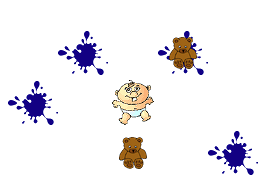
\includegraphics[height=4.5cm]{Teddy.png}
\end{figure}
\vspace{2cm}}

\author{\textbf{Benötigte IDEs:}\\
\href{https://www.greenfoot.org/}{Greenfoot}, \href{https://www.bluej.org/}{BlueJ}
\vspace{2cm}}

\date{\textbf{Verfasser:}\\
\href{https://nikothegreek.jimdofree.com/}{Niko Diamadis}\\
\vspace{0.5cm}
\textbf{Erstellungs-/ Änderungsdatum}\\
\today\enlargethispage{4cm}}
%----------------------------------------------------------------------------------------

%----------------------------------------------------------------------------------------
%   2. SEITE
%----------------------------------------------------------------------------------------
\doublespacing

\maketitle\thispagestyle{empty}

\numberwithin{equation}{section}
\cleardoublepage

\setcounter{page}{1}
\tableofcontents
%----------------------------------------------------------------------------------------


%----------------------------------------------------------------------------------------
%   3. UND NACHFOLGENDE SEITEN
%----------------------------------------------------------------------------------------
\newpage
\pagenumbering{arabic}  % Ändern der Seitenangabe

\cleardoublepage

\section{Das Spiel}

\subsection{Vorbereitungen}

Zu dieser Aufgabe sind meines Erachtens nach keine Anleitungen und/oder Erläuterungen nötig.\\
Wenn doch Fragen aufkommen, schreib' einfach an \textbf{\href{mailto:nikodiamond3@gmail.com}{nikodiamond3@gmail.com}}.

\subsection{Basis-Teddy}

Anhand des Quellcodes ist zu erkennen, dass folgende Attribute und Methoden einem Teddy schon zugeordnet sind:

\begin{itemize}
    \barrow Attribute
    \begin{itemize}
    \item sämtlichte Attribute der Überklasse Actor (\texttt{class Teddy extends Actor})
    \end{itemize}
    \barrow {Methoden}
    \begin{itemize}
    \item \texttt{springen} ohne Rückgabewert und ohne Parameter (\texttt{void springen()})
    \item sämtlichte Methoden der Überklasse Actor (\texttt{class Teddy extends Actor})
    \end{itemize}
\end{itemize}

\subsection{Attribute}

\begin{figure}[ht]
	\centering
	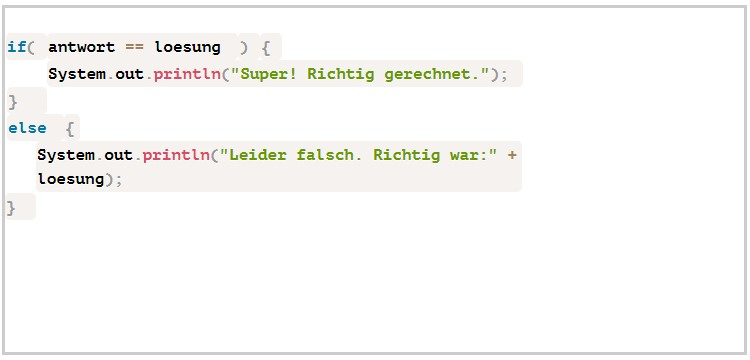
\includegraphics[height=1.5cm]{2.3.1.2/1.Das_Spiel/3-1.png}
\end{figure}

Im Objektinspektor sind wie erwartet die Attribute \texttt{leben} und \texttt{alter} wiederzufinden, es hat demnach alles geklappt.

\newpage

\subsection{Syntaxfehler}

\begin{figure}[ht]
	\centering
	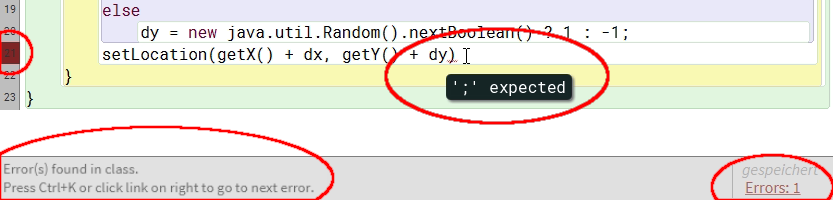
\includegraphics[height=3.4cm]{2.3.1.2/1.Das_Spiel/4-1.png}
\end{figure}

In Greenfoot sind Syntaxfehler im Quellcode wie im Bild zu sehen an vier Stellen erkennbar:

\begin{itemize}
    \barrow rot markierte Zeilenangaben
    \barrow rot unterstrichener Teil des Quellcodes und Fehlerbeschreibung
    \barrow Fehlermeldung und Angabe, wie man schnell zum Fehler gelangt (Strg + K oder Klick auf Meldung unten rechts)
    \barrow Angabe der Fehleranzahl unten rechts in der Ecke
\end{itemize}

\subsection{Konstruktor}

Zu dieser Aufgabe sind meines Erachtens nach keine Anleitungen und/oder Erläuterungen nötig.\\
Wenn doch Fragen aufkommen, schreib' einfach an \textbf{\href{mailto:nikodiamond3@gmail.com}{nikodiamond3@gmail.com}}.

\subsection{act}

Es gibt mehrere Arten, die Variable um 1 zu erhöhen:

\textbf{1. (funktioniert auch mit komplexeren Rechnungen)}
\begin{lstlisting}
public void act() {
    alter = alter + 1;
}
\end{lstlisting}

\textbf{2. (funktioniert auch bei Addition mit anderen Zahlen)}
\begin{lstlisting}
public void act() {
    alter += 1;
}
\end{lstlisting}

\textbf{3. (funktioniert nur für Addition mit 1)}
\begin{lstlisting}
public void act() {
    alter++;
}
\end{lstlisting}

\subsection{verringereLeben}

\begin{lstlisting}
public void verringereLeben(int betrag) {
    leben = leben - betrag;
}
\end{lstlisting}

\subsection{Wert}

\begin{itemize}
    \barrow In der Methode \texttt{getWert} ist als Rückgabewert \texttt{int} festgelegt.\\
    Der zurückzugebene Wert ergibt sich aus Abziehen des Wertes des Attributs \texttt{alter} von 100.
    \barrow In der Methode \texttt{hatWert} ist als Rückgabewert \texttt{boolean} festgelegt.\\
    Wenn der zurückzugebene Wert der Methode \texttt{getWert} größer als 0 ist, gibt diese Methode \texttt{true} zurück, andernfalls wird \texttt{false} zurückgegeben.
\end{itemize}

\subsection{Spiel fertig stellen}

Zu dieser Aufgabe sind meines Erachtens nach keine Anleitungen und/oder Erläuterungen nötig.\\
Wenn doch Fragen aufkommen, schreib' einfach an \textbf{\href{mailto:nikodiamond3@gmail.com}{nikodiamond3@gmail.com}}.

\newpage

\section{Fachkonzept - OOM}

Zu dieser Seite sind meines Erachtens nach keine Anleitungen und/oder Erläuterungen nötig.\\
Wenn doch Fragen aufkommen, schreib' einfach an \textbf{\href{mailto:nikodiamond3@gmail.com}{nikodiamond3@gmail.com}}.

\newpage

\section{Fachkonzept - OOP}

Zu dieser Seite sind meines Erachtens nach keine Anleitungen und/oder Erläuterungen nötig.\\
Wenn doch Fragen aufkommen, schreib' einfach an \textbf{\href{mailto:nikodiamond3@gmail.com}{nikodiamond3@gmail.com}}.

\newpage

\section{Übungen}

\subsection{Struktur von Klassen}

\begin{figure}[ht]
	\centering
	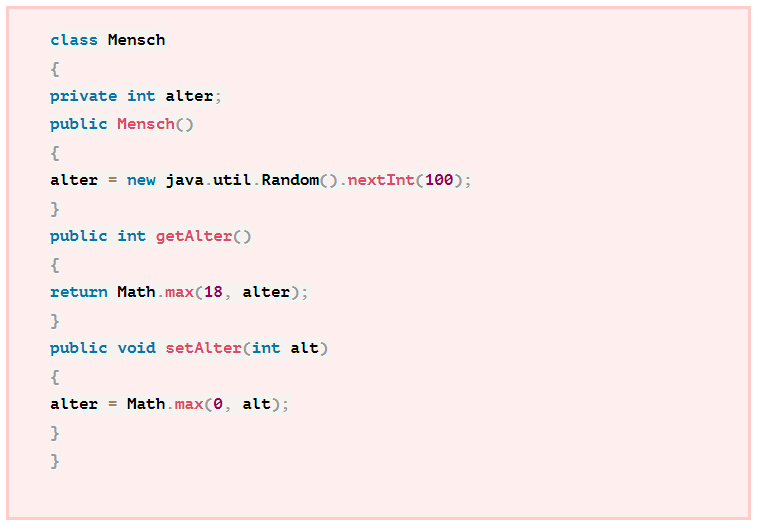
\includegraphics[height=9cm]{2.3.1.2/4.Uebungen/1-1.png}
\end{figure}

\subsection{Eine Würfel-Klasse}

\begin{figure}[ht]
	\centering
	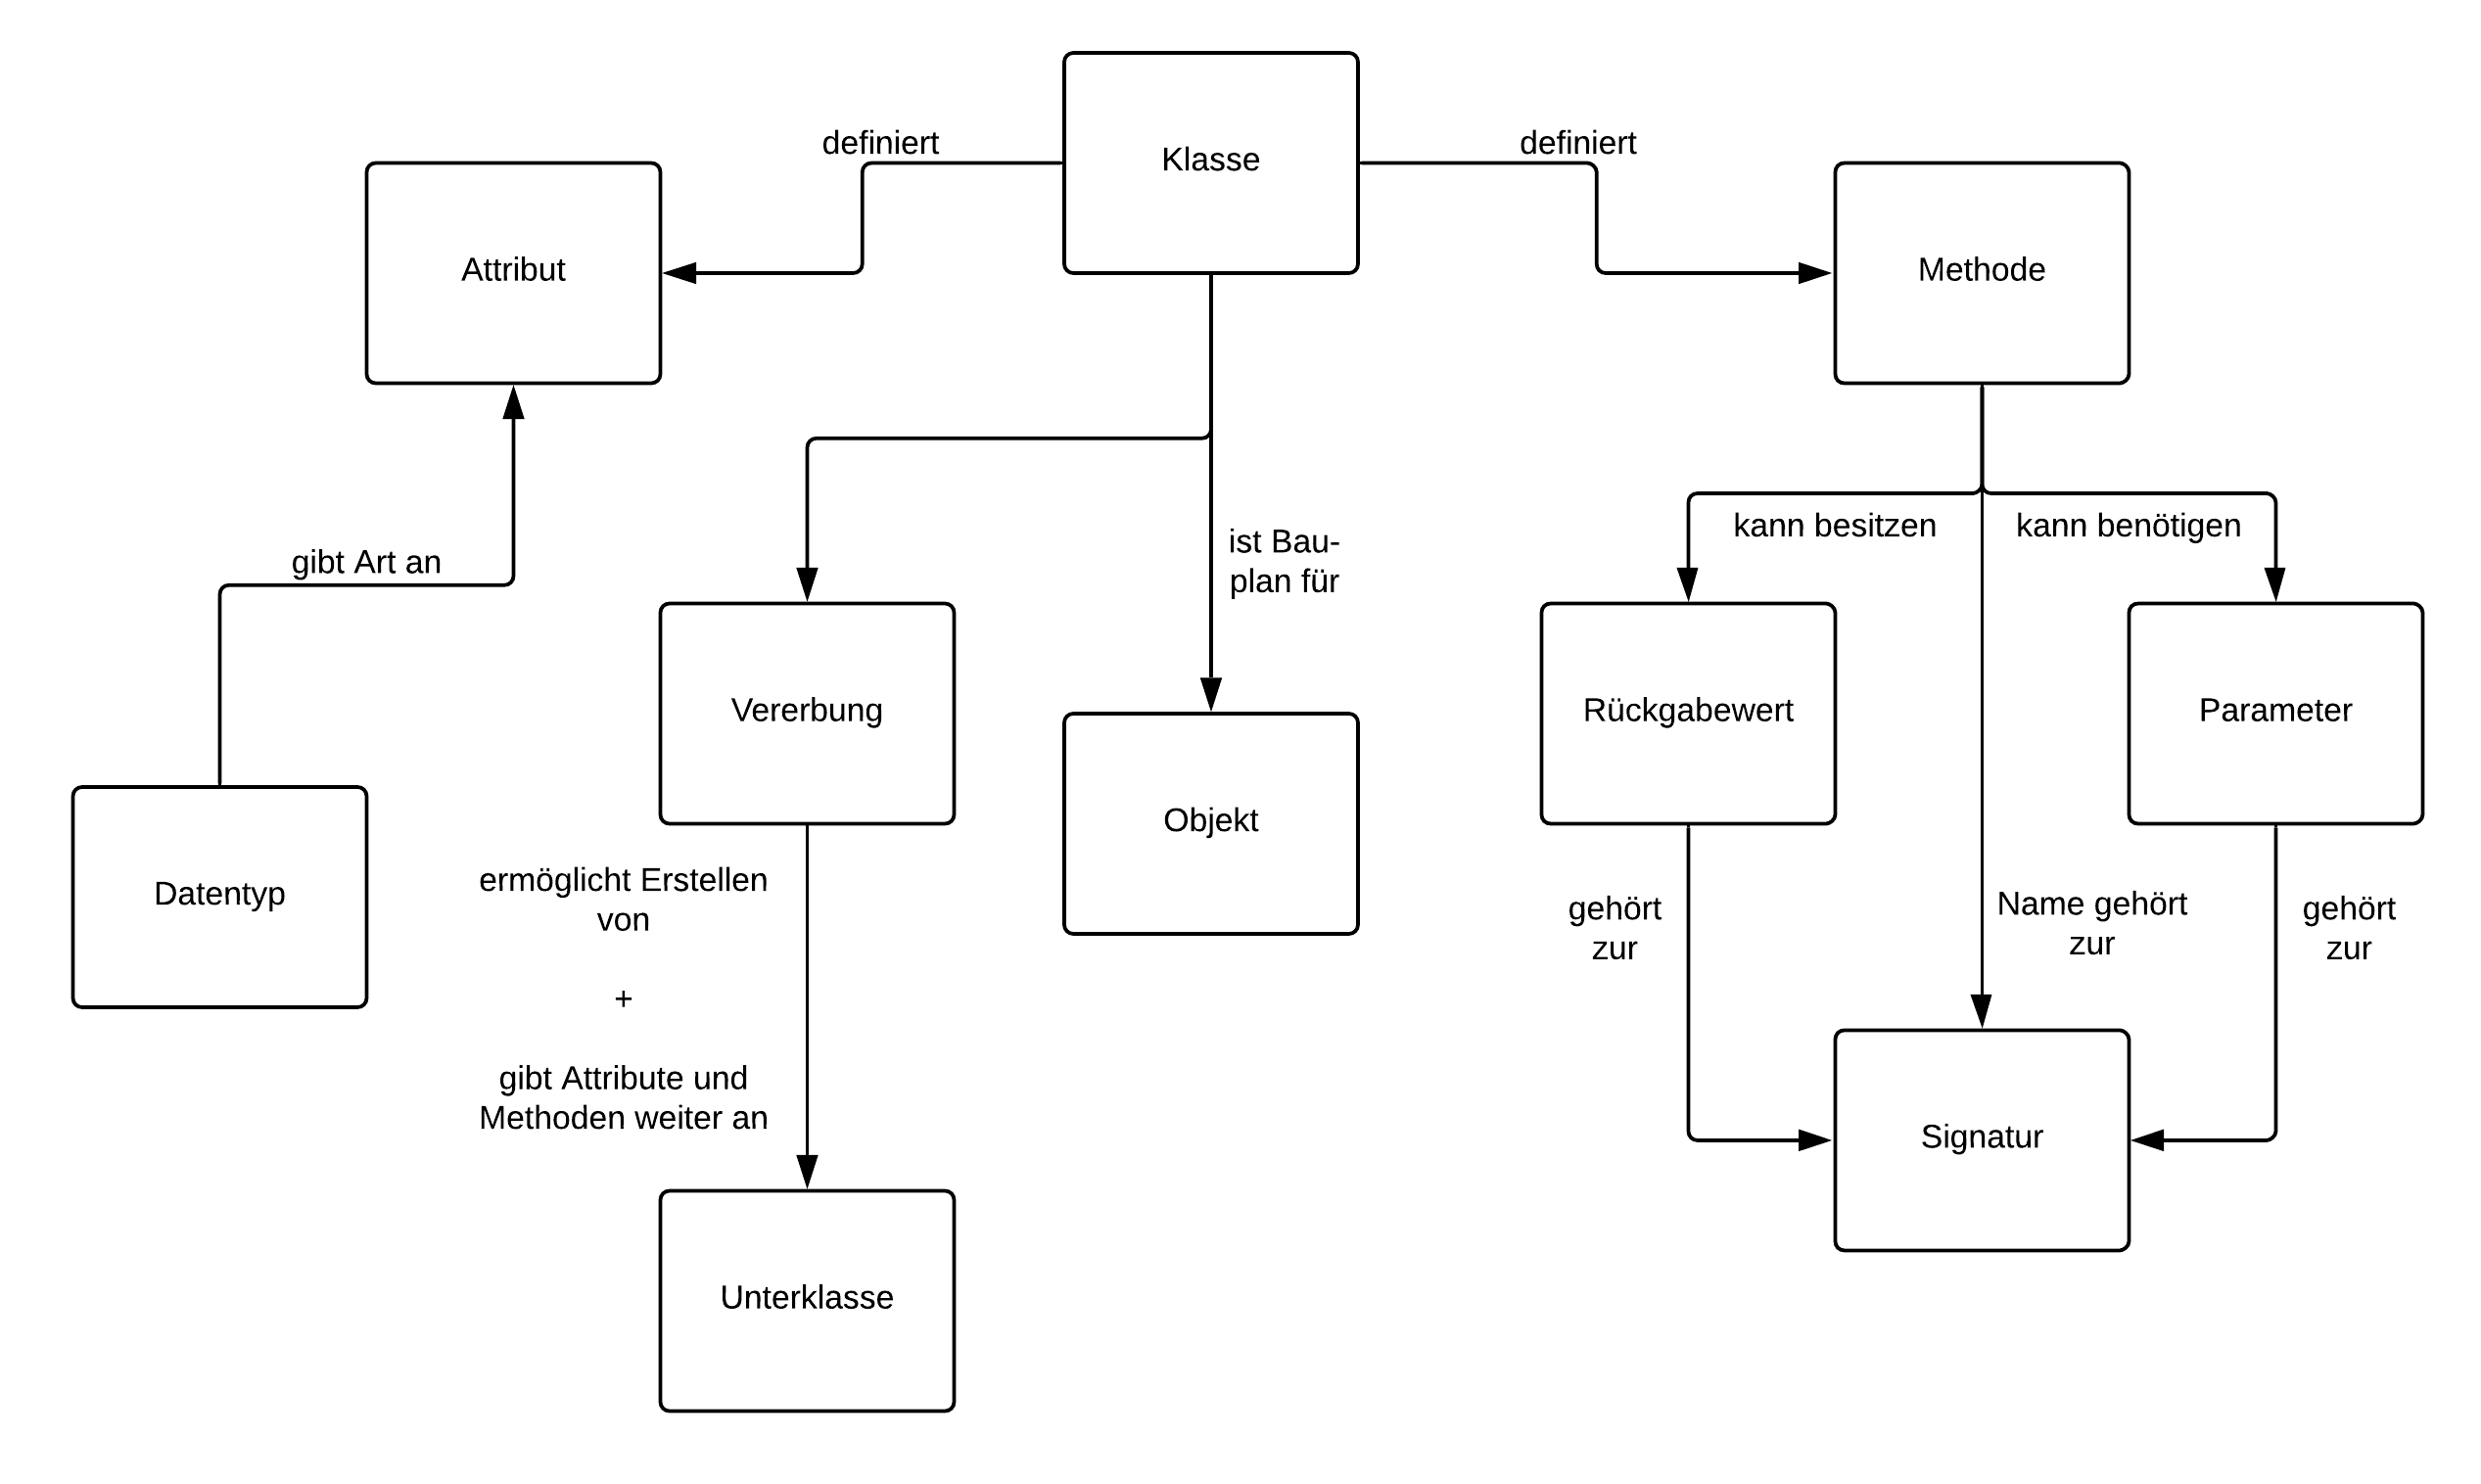
\includegraphics[height=5cm]{2.3.1.2/4.Uebungen/2-1.png}
\end{figure}

Wir erstellen nur eine Methode, welche man selber aufrufen kann und welche im Konstruktor aufgerufen wird. Diese Methode soll dem Würfel eine Zahl von 1 bis 6 zuweisen.

\newpage

\begin{lstlisting}
public class Wuerfel {
    int augenzahl;
    
    Wuerfel() {
        wuerfeln();
    }
    
    void wuerfeln() {
        augenzahl = new java.util.Random().nextInt(6) + 1;
    }
}
\end{lstlisting}

Der Ausdruck \texttt{new  java.util.Random().nextInt(6)} bewirkt, dass eine Zufallszahl von 0 bis 5 erstellt wird, da ein Würfel aber die Augenzahlen 1 bis 6 besitzt, addieren wir einfach 1.

\subsection{Eine Klasse für Brüche}

Im Vorhinein ist noch zu sagen, dass ich (wie vielleicht schon erkannt) Freund von kurzem Code bin (siehe \hyperlink{subsection.1.6}{\textbf{1.6}}). Daher bevorzuge ich die dort auch schon angesprochene Schreibweise (wenn der Summand größer als 1 ist):\\
\begin{lstlisting}
alter += 1;
\end{lstlisting}

In dieser Aufgabe sind aber Multiplikationen und Divisionen gefordert. Die einfache Schreibweise ähnelt der ersten Schreibweise bei \hyperlink{subsection.1.6}{\textbf{1.6}}.\\
Wenn wir nun aber die Schreibweise vereinfachen wollen, können wir bei der zweiten Schreibweise von \hyperlink{subsection.1.6}{\textbf{1.6}} das \glqq +\grqq{} durch ein \glqq *\grqq{} bzw. ein \glqq/\grqq{} ersetzen, womit Multiplikationen und Divisionen mit dem dann folgenden Faktor bzw. Divisor ausgedrückt werden.\\

Nun zurück zur Aufgabe...

\newpage

\begin{lstlisting}
public class Bruch {
    int zaehler;
    int nenner;
    
    Bruch(int z, int n) {
        zaehler = z;
        nenner = n;
    }
    
    void erweitern(int k) {
        zaehler *= k;
        nenner *= k;
    }
    
    void kuerzen(int k) {
        zaehler /= k;
        nenner /= k;
    }
}
\end{lstlisting}

Wenn man Brüche zu kürzen versucht, die nicht mehr zu kürzen sind, dann werden Zähler und Nenner jeweils mit dem Faktor dividiert und das Ergebnis jeweils gerundet.\\
In diesem Falle ist dann das Ergebnis folglich falsch!

\subsection{Ein objektorientiertes Modell herleiten}

Hier gebe ich keine Lösungsansätze bzw. Lösungen, da es sich jeder unterschiedlich vorstellt, wie ein Autorennen im Computer aussehen soll. Hier kann man seinen Ideen freien Lauf lassen.\\
Solange man sich an die richtige Syntax hält, kann bei dieser Aufgabe nichts falsch gemacht werden.

\newpage

\section{Übungsprojekt - Autobewertung}

\subsection{Ein mathematisches Modell für ein Auto finden}

Man erkennt hoffentlich schnell, dass es z.B. eine Exponentialfunktion sein kann.\\
Wenn man dann in die allgemeine Funktionsvorschrift verschiedene Werte unter 1 als Basis eingibt und die resultierenden Graphen mit dem auf inf-schule vergleicht (und entsprechend die Basis anpasst), kommt man ungefähr zu folgender Funktion:

\begin{center}
    \texttt{$f(alter) = neupreis * 0,87^{ alter}$}
\end{center}

Die Funktion muss die y-Achse schneiden, da der y-Achsenabschnitt in unserem Falle den Neupreis des Autos darstellt.

\subsection{Ein objektorientiertes Modell für ein Auto finden}

\begin{itemize}
    \barrow \texttt{neupreis : int}\\
    ganzzahliger Preis (aufgrund von genereller Ungenauigkeit reicht die Angabe in \euro)
    \barrow \texttt{alter : double}\\
    Alter als Gleitkommazahl, da das Alter in Jahren angegeben wird, man aber auch die Angabe in kleineren Schritten ermöglichen möchte
    \barrow Die Methoden haben alle als Rückgabewert \texttt{double}, da mit dem Attribut \texttt{alter} gerechnet wird, welches vom Datentypen \texttt{double} ist, es kommen also Ergebnisse mit Nachkommastellen heraus, welche z.B. mit dem Datentyp \texttt{int} nicht darzustellen sind.
    \barrow Die Methoden benötigen keine Parameter, da die Attribute in allen Methoden benutzt werden, also die Angabe der Attribute methodenunabhängig getätigt wird, sodass nicht bei jedem Aufruf einer Methode z.B. der Neupreis angegeben werden muss. Die Methoden greifen auf die klassenweiten Attribute zu.
\end{itemize}

\newpage

\subsection{Ein Automodell objektorientiert implementieren}

\begin{itemize}
    \barrow Kriegst du hin, oder? Du musst nur den Code aus dem Video kopieren.
    \barrow Bisher wird von beiden Methoden nur der Wert \texttt{0} ausgegeben, da weder \texttt{neupreis} noch \texttt{alter} einen Wert von uns zugewiesen bekommen haben.
    \barrow Das \texttt{return} und der danach folgende Ausdruck gibt an, welchen Wert die Methode zurückgeben soll.
    \barrow Der Ausdruck \texttt{Math.pow(0.87, alter)} ist die Umschreibung einer Potenz im Java-Code (\texttt{pow} für \glqq power\grqq{} (englisch für Potenz). Der erste angegebene Wert ist die Basis und der zweite Wert (mit Komma getrennt) stellt den Exponenten dar.
    \barrow Mit \texttt{return neupreis - getMarktwert()} gibt die entsprechende Methode als Rückgabewert die Differenz von \texttt{neupreis} und dem Rückgabewert der \texttt{getMartkwert}-Methode zurück.
    \barrow Versteht man glaube ich schnell, wenn man es sieht...\\
    \begin{lstlisting}
double getHaendlerEk() {
    return getMarktwert() * 0.8;
}
\end{lstlisting}
\end{itemize}
    
\subsection{Objekte initialisieren}

\begin{itemize}
    \barrow Keine Anleitungen und/oder Erläuterungen nötig...
    \barrow \vspace{15pt}
    \begin{tabular}[ht]{c|c}
\\\textbf{Gemeinsamkeiten} & \textbf{Unterschiede}\\
\hline
Parameter & Konstruktor kann keinen Wert zurückgeben\\
\hline
& Konstruktorname entspricht immer dem Klassennamen\\
\hline
& Konstruktor nur einmalig vor allen Methoden aufrufbar\\
\end{tabular}
\end{itemize}

\subsection{Attributwerte verändern}

Zu dieser Aufgabe sind meines Erachtens nach keine Anleitungen und/oder Erläuterungen nötig.\\
Wenn doch Fragen aufkommen, schreib' einfach an \textbf{\href{mailto:nikodiamond3@gmail.com}{nikodiamond3@gmail.com}}.

\subsection{Erweiterung des Klassendiagramms}

\begin{figure}[ht]
	\centering
	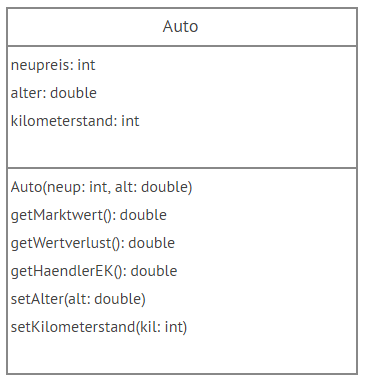
\includegraphics[height=7.5cm]{2.3.1.2/5.Uebungsprojekt-Autobewertung/6-1.png}
\end{figure}

\subsection{Erweiterung der Implementierung}

Wir geben, wie vorgeschlagen, den Kilometerstand in \glqq Tausend Kilometern\grqq{} an, sodass ich durch Ausprobieren grob auf folgende Basis kam:

\begin{center}
    \texttt{$f(kilometerstand) = neupreis * 0,995^{kilometerstand}$}
\end{center}

In den Code implementiert könnte es z.B. so aussehen:

\begin{lstlisting}
int kilometer;

Auto(int neup, double alt, int kil) {
    neupreis = neup;
    alter = alt;
    kilometer = kil;
}

double getMarktwert() {
    return neupreis * Math.pow(0.87, alter) * Math.pow(0.995, kilometer);
}
void setKilometerstand(int kil) {
    kilometer = kil;
}
\end{lstlisting}

\subsection{Eigene Ideen}

Hier lasse ich deinen Ideen mal freien Lauf, viel Spaß beim Implementieren und Ausprobieren!\\
Bei Fragen einfach an \textbf{\href{mailto:nikodiamond3@gmail.com}{nikodiamond3@gmail.com}} schreiben.

\subsection{Grenzen von Modellen}

Das bisher benutzte Modell passt nur zu Autos in der Preisklasse des VW Golfs und im selben Zustand wie dieser (also ohne große Schäden o.Ä.), andere teurere oder billigere Autos würden einen anderen Faktor aufweisen.

Außerdem funktioniert die Modellierung des Werteverlustes nicht unendlich lange, irgendwann werden Autos z.B. wieder wertvoller (wenn der Zustand dementsprechend ist).

Verbessern könnte man auch noch die Rückgabewerte der Methoden, da diese sehr viele Nachkommastellen besitzen können, was im Kontext wenig Sinn ergibt. Ich verschone dich aber lieber mit Funktionen zum Runden.

\end{document}